\documentclass[12pt]{report}
\usepackage[margin=0.5in]{geometry}
\usepackage{amsmath}
\usepackage{nccmath}
\usepackage{alltt}
\usepackage{sectsty}
\usepackage{titlesec}
\newcommand{\ts}{\textsuperscript}
\usepackage{graphicx}
\graphicspath{ {../images/} }

\titlespacing*{\section}{0pt}{0.8\baselineskip}{0.2\baselineskip}

\begin{document}

\begin{titlepage}
    \begin{center}
        \vspace*{1cm}
        
        \textbf{CO3093 COURSEWORK 1 Report}
        
        \vspace{0.5cm}
		Big Data \& Predictive Analytics - Simulation-based \& Regression Models
        
        \vspace{1.5cm}
        
        \textbf{Ihtasham Chaudhry}
        
        \vfill
        
        \vspace{0.8cm}
                
        Department of Informatics\\
        University of Leicester\\
        23\ts{rd} February 2018
        
    \end{center}
\end{titlepage}

\newpage

\section{Question 1}

\vspace{0.5cm}

\subsection{1.1}

\vspace{0.5cm}

It is important to consider missing values in our data set and to filter out the columns based on this information so that we have all the information we need to make predictions and have \emph{clean} data. In the case of our problem (predicting a winner), the most important factors that we must consider are win/loss statistics and goals scored/conceded statistics.

\noindent
We can then draw some conclusions from the data such as:
\begin{enumerate}
	\item The average number of goals scored per match throughout the tournament by each team playing at home is 1.49 and away is 1.18. We also notice that the median of these values falls close to the minimum values which indicates that the data on this column is positively skewed and has a longer tail towards higher values.
	\item From this data we can also observe that on average teams win more games playing home than they do playing away, The mean ($\mu$) of wins at home for each team is larger than the median of the dataset, this indicates that the distribution is skewed towards large values. The standard deviation ($\sigma$) is very small relative to the min and max values, this indicates that the distribution has "long tails". 
	 \item Following from the previous point, the same observation can be made regarding the number of "FTHG" or "Full Time Home Goals" by each team per match. The data again is skewed towards larger values. 
	 
\end{enumerate}

\subsection{1.2}
\noindent
As we are only considering two teams; Manchester United and Manchester City, we can further filter the data and extract only the games played by both of those teams where they are playing either home or away. When we accumulate the data by teams and their home and away games to see how they perform for each category. After doing this we can draw some analysis from the data.

\vspace{0.3cm}
\noindent

\iffalse
\begin{table}[ht]
\centering
\caption{Full time results over the season (higher is better)}
\begin{tabular}{lllll}
         & Wins & Losses & Draws &  \\
Man Utd  & 16 & 3 &  5 & \\
Man City & 21 & 1 & 2 &\\

\end{tabular}
\end{table}
\fi

\begin{table}[ht]
\centering
\caption{Mean goals scored per game over the season (higher is better)}
\begin{tabular}{lllll}
         & Home & Away &  &  \\
Man Utd  & 2.25 & 1.83 &  &  \\
Man City & 3.50 & 2.33 &  &  \\
\end{tabular}
\end{table}

\begin{table}[ht]
\centering
\caption{Mean goals conceded per game over the season (lower is better)}
\begin{tabular}{lllll}
         & Home & Away &  &  \\
Man Utd  & 0.41 & 0.91 &  &  \\
Man City & 0.75 & 0.75 &  &  \\
\end{tabular}
\end{table}

\noindent
We can see that over 24 games played by both teams over the course of the season, Man City has a higher average of goals both in the home and away side compared to Manchester United, and have conceded a higher average of goals home but a lesser average of goals home compared to Manchester United. 

\newpage

\subsection{1.3}
\vspace{0.3cm}
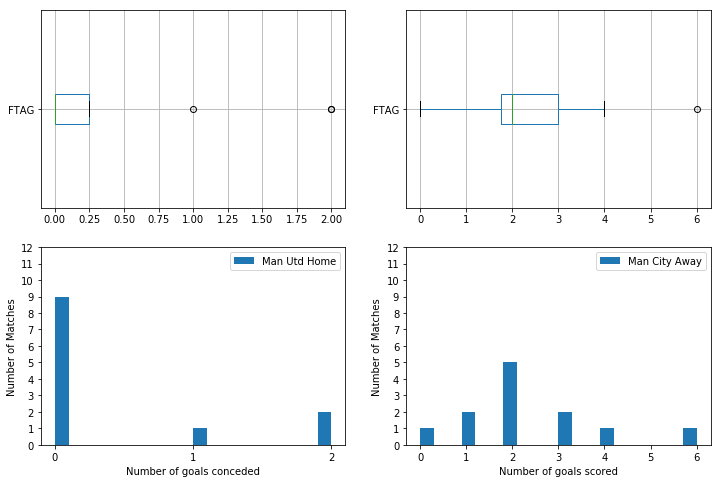
\includegraphics[scale=0.7]{fig1}

\end{document}